\chapter{記分板}
\section{繪圖}
\begin{figure}[h]
  \centering
  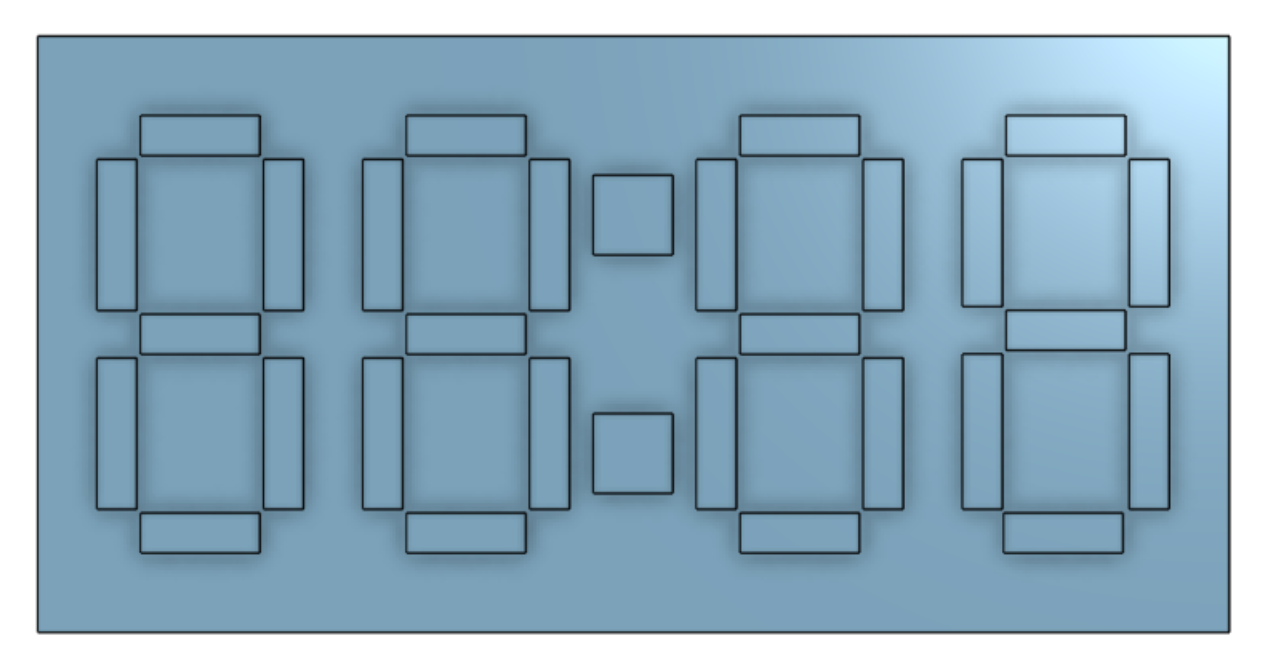
\includegraphics[width=0.5\textwidth]{計分板繪圖_17.png}
  \caption{LED記分板\_1}
  \label{fig:photo1}
\end{figure}

\begin{figure}[h]
  \centering
  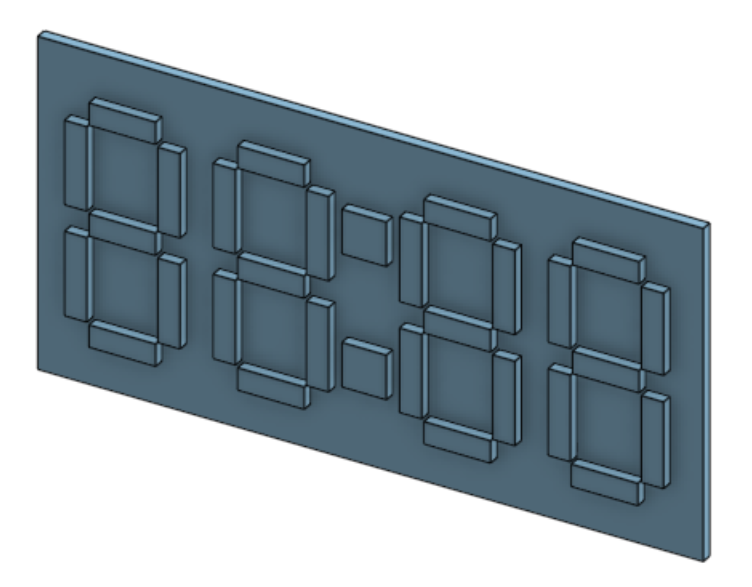
\includegraphics[width=0.5\textwidth]{計分板繪圖_18.png}
\end{figure}

\begin{figure}[h]
  \centering
  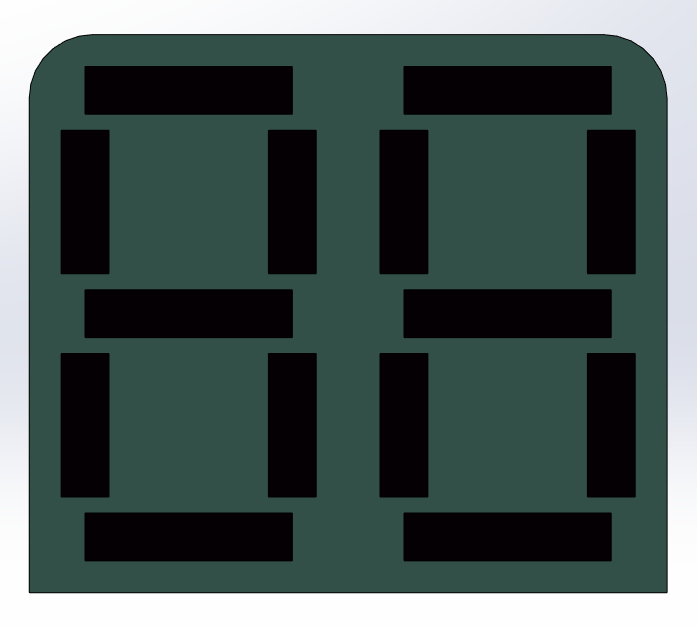
\includegraphics[width=0.5\textwidth]{計分板繪圖_15.png}
  \caption{LED記分板\_2}
  \label{fig:photo2}
\end{figure}

\begin{figure}[h]
  \centering
  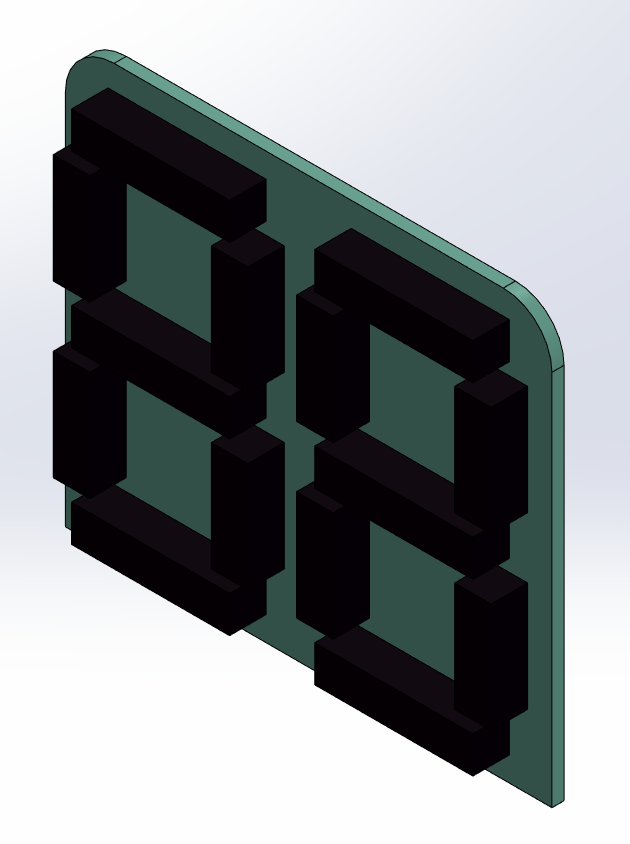
\includegraphics[width=0.5\textwidth]{計分板繪圖_16.png}
\end{figure}
\newpage
\section{組合}
 取自 1977年發行的一款家用遊戲機ATARI 2600中的遊戲,內建於Gym,這是一個橫向的乒乓遊戲,左方是預設電腦玩家,右邊由使用者或是由訓練程式控制(圖.\ref{fig.pong})。在強化學習範例中,Pong與實體冰球機簡化後環境相似。\\

\section{組裝}

\newpage
